My parents put me through three divorces. My mother and father divorced when I was very young. Young to the point where I don't remember them being married. I remember finding a picture of them walking with their arms around each other's backs. Dad was shirtless and chestnut brown, hair a near-black 'fro. Mom was in a white blouse, blonde hair in a perm. It seemed so alien to me.

Mom and Jay got divorced when I was in my freshman year of high school. I remember being taken to a family therapy session for Jay's lingering divorce with his previous wife, but no such luck with his divorce with my mom. I just remember things getting bad after I came out, and then my mom coming downstairs to wake me one morning and inform me that we were moving out. Today. Now.

I don't remember ever seeing Jay again after that, though I surely must have.

\begin{quote}
But you heard about him.
\end{quote}

Mom said he called Erin, my ex-step-sister a ``witch''. I don't think that's the word he used. A decade and a half later, she'd suggest that I go visit him.

I turned her down.

\begin{quote}
A sub-story. Do I sense conflict?
\end{quote}

Of course.

\begin{quote}
You may be made of star-stuff, but conflict seems to be what holds you together.
\end{quote}

Stop trying to get me to talk about mania.

At first, I was proud of my relationships. Then I was embarrassed. There were so many, all in a line. One would trickle into existence with, as I put it, \texttt{light,\ in\ through\ the\ head,\ out\ through\ the\ heart}. We'd be perfect, until we weren't. Everything would be delightful, until it wasn't. It's the way of early relationships, I suppose. You fall for someone, and you can't quite pick apart the difference between love and lust.

I just went through so many that I started feeling a bit weird about it. How do I talk about the Danny-Marek-Merlin-Andrew-Michael-Andy-Rikky-Kayla-Tyson-Andrew(again) progression? And how do I talk about Lon? Or what JD and I were at the beginning?

\begin{quote}
Doubtless with the same lilac-scented words you talk about everything.
\end{quote}

I guess.

Early on, I promised myself that I would do anything to not become my dad, in so many ways. One of those was to not run my relationships like him. Some bits were easy, of course. I could start by being queer. That's glib, of course, but at the time I started dating, being queer required more discretion, more discussion than I saw in my dad's relationships.

Some bits weren't so easy, though. The overlap between the discussion that's involved the mechanics of simply having a queer relationship and the discussion that's involved in having a healthy relationship, queer or not, is not non-existent, but neither is it large.

\begin{quote}
Are you going to provide us with a Venn Diagram? In hand-coded SVG, perhaps?
\end{quote}

\href{/healthy-sound.svg}{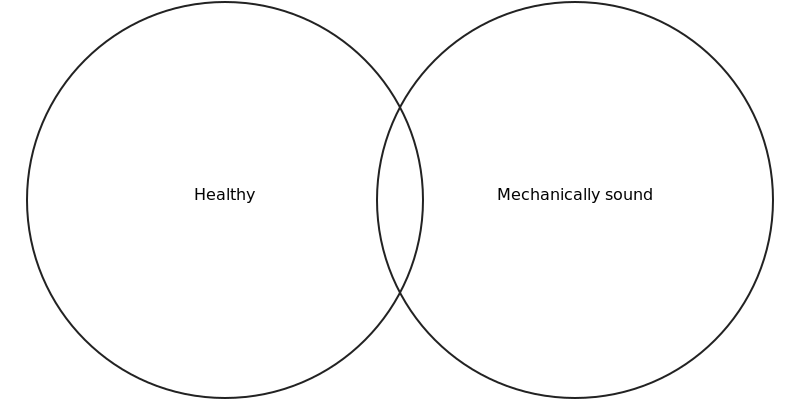
\includegraphics{/healthy-sound.svg}}

Happy?

\begin{quote}
Very. I just wanted to ensure that you were at your very Maddy-est about this.
\end{quote}

When my dad divorced Julie, he told her he hadn't loved her in ten years. He told her he married her because she was easy to deal with. Quiet. Compliant. Not as smart as him. He could be right around her, which wasn't always guaranteed with mom.

Julie's friends gave her a rubber rat afterward. They had scribbled his name on it. The rat was sitting on a plaque that said \texttt{Rat\ Bastard}. The last time I saw her, she was very drunk, sagged against my side, sobbing and beating that rat against the nightstand.

\begin{quote}
And you didn't want to be like him when you grew up? Color me surprised.
\end{quote}

You \emph{would} say that.

He had started dating well before divorcing her. I don't know if he and Maurine are married now. When I told mom, she shrugged and said that he had started dating Julie before their own divorce.

\begin{quote}
You dovetailed relationships. You were dating Andrew well before you and Tyson fell away from each other.
\end{quote}

Hey, I said some bits weren't as easy. He left me with a lot of him in me.

\begin{quote}
Like the anger. He gave you that. The anger and the pride.
\end{quote}

I pay for his past as well as mine.

So, when Michael mentioned that he wanted to go on a date with someone else while we were together, well, it touched a nerve.
